\documentclass[a4paper,11pt,twocolumn]{article}
\usepackage[utf8]{inputenc}
\usepackage[T5]{fontenc}

\usepackage{mathptmx}
\usepackage{geometry}
\usepackage{graphicx}
\usepackage{amsmath}
\usepackage{amssymb}
\usepackage{amsfonts}
\usepackage{float}
\usepackage{indentfirst}

\usepackage[english,vietnamese]{babel}
\usepackage[utf8]{inputenc}
\usepackage[T5]{fontenc}

\setlength{\parindent}{15pt}

\renewcommand{\thesection}{\Roman{section}.}
\renewcommand{\thesubsection}{\arabic{section}.\arabic{subsection}}
\addto\captionsvietnamese{
	\renewcommand{\figurename}{Figure}
	\renewcommand{\tablename}{Table}
}

\geometry{
	a4paper,
	left=20mm,
	right=20mm,
	top=22mm,
	bottom=20mm,
	columnsep=7mm
}

\title{\bfseries Building an Adaptive Vietnamese License Plate Recognition and Retrieval System using Multi-Task Deep Learning}

\author{
	Phuoc Minh Hieu PHAM$^{1}$, Sy Sieu CAO$^{1}$, Le Phu Trung HUYNH$^{1*}$\\
	$^{1}$University of Management and Technology HCMC\\[4pt]
	*Corresponding author: trung.huynhlephu@umt.edu.vn
}
\date{}

\begin{document}
	
	\twocolumn[
	\maketitle
	
	\selectlanguage{english}
	\renewcommand{\abstractname}{Abstract}
	
	\begin{abstract}
		Automatic License Plate Recognition (ALPR) is an essential component of intelligent transportation, yet its performance is often significantly degraded by real-world image distortions and regional plate format complexities. This research addresses these challenges by proposing a highly adaptive, multi-task deep learning framework specifically designed for the Vietnamese license plate context. The system targets the unique diversity of Vietnamese plates while robustly handling low-quality image inputs through a multi-stage, conditional pipeline. First, a real-time object detection model localizes all license plate instances. The core component is a lightweight Quality Assessment Module (QAM), which acts as an intelligent router, classifying each plate as ``clear'', ``restorable'', or ``unrestorable''. Based on this assessment, ``restorable'' images are selectively forwarded to a Swin2SR-based restoration network, while ``clear'' images bypass this step to optimize throughput, and ``unrestorable'' inputs are discarded. Finally, a Transformer-based Optical Character Recognition (OCR) model transcribes the characters to retrieve vehicle information. Experimental evaluations confirm the effectiveness of this end-to-end adaptive strategy, achieving a Character Accuracy of 96.07\% and a Sequence Accuracy of 89.69\%. These results demonstrate significant robustness against real-world distortions compared to traditional monolithic pipelines, offering a practical and efficient solution for ALPR applications in Vietnam.
	\end{abstract}
	
	\vspace{0.5em}
	\noindent\textbf{\small Keywords—} Vietnamese License plate recognition, multi-task learning, computer vision.
	
	\selectlanguage{vietnamese}
	\renewcommand{\abstractname}{Tóm tắt}
	\begin{abstract}
		Nhận dạng biển số xe tự động (ALPR) là một thành phần trọng yếu trong hệ thống giao thông thông minh. Tuy nhiên, hiệu suất của các hệ thống này thường bị suy giảm nghiêm trọng do sự biến dạng của hình ảnh trong môi trường thực tế và sự phức tạp về định dạng biển số đặc thù của từng khu vực. Nghiên cứu này giải quyết các thách thức trên bằng cách đề xuất một khung kiến trúc học sâu đa nhiệm có khả năng thích ứng cao, được thiết kế chuyên biệt cho bối cảnh biển số xe tại Việt Nam. Hệ thống hướng tới việc xử lý sự đa dạng của biển số Việt Nam đồng thời giải quyết triệt để các đầu vào hình ảnh chất lượng thấp thông qua một quy trình xử lý phân tầng có điều kiện. Đầu tiên, một mô hình phát hiện vật thể thời gian thực được sử dụng để định vị tất cả các biển số xe. Thành phần cốt lõi của hệ thống là Mô-đun Đánh giá Chất lượng hạng nhẹ, hoạt động như một bộ định tuyến thông minh để phân loại từng biển số thành ba nhóm: "rõ nét", "có thể phục hồi", hoặc "không thể phục hồi". Dựa trên kết quả đánh giá này, các ảnh "có thể phục hồi" sẽ được điều hướng có chọn lọc qua mạng phục hồi ảnh sử dụng kiến trúc Swin2SR, trong khi các ảnh "rõ nét" sẽ bỏ qua bước này để tối ưu hóa tốc độ xử lý, và các ảnh "không thể phục hồi" sẽ bị loại bỏ. Cuối cùng, một mô hình Nhận dạng Ký tự Quang học dựa trên kiến trúc Transformer được sử dụng để nhận dạng chuỗi ký tự nhằm truy xuất thông tin phương tiện. Các đánh giá thực nghiệm đã khẳng định tính hiệu quả của chiến lược thích ứng đầu cuối này, đạt độ chính xác theo ký tự là 96.07\% và độ chính xác theo chuỗi là 89.69\%. Những kết quả này chứng minh khả năng hoạt động bền vững và vượt trội trước các biến dạng thực tế so với các mô hình xử lý tuyến tính truyền thống, mang lại một giải pháp thực tiễn và hiệu quả cho các ứng dụng ALPR tại Việt Nam.
	\end{abstract}
	
	\vspace{0.5em}
	\noindent\textbf{\small Từ khóa—} Nhận dạng biển số xe Việt Nam, học đa tác vụ, thị giác máy tính.
	
	\vspace{1em}
	]
	
	
	\section{INTRODUCTION}
	
	Automatic License Plate Recognition (ALPR) serves as a cornerstone technology within modern Intelligent Transportation Systems (ITS). Its applications are extensive and critical, underpinning systems for automated toll collection, traffic law enforcement, smart parking management, and vehicle access control. The efficacy of these applications hinges on the system's ability to provide accurate and real-time vehicle identification.
	
	However, the performance of conventional ALPR systems degrades significantly when deployed in unconstrained real-world environments. These systems often fail when faced with a wide spectrum of image quality issues, including motion blur from fast-moving vehicles, severe glare from headlights or sunlight, low-light noise, and geometric distortions from oblique camera angles.
	
	This research specifically addresses the challenges within the Vietnamese license plate context. This environment presents unique regional complexities, including a high diversity of plate formats, various background colors (e.g., white, blue, yellow), and differing character layouts. A "one-size-fits-all" ALPR solution is often insufficient to handle this variability, leading to high error rates.
	
	\section{RELATED WORK}
	
	The proposed system comprises four sequential yet adaptive stages: (1) license plate detection, (2) image quality assessment and routing, (3) conditional image restoration, and (4) character recognition and retrieval.
	
	\subsection{\textit{License Plate Detection Challenges}}
	
	Recent years have witnessed significant strides in object detection, particularly with the evolution of one-stage detectors like the YOLO family, which have revolutionized real-time applications by achieving high inference speeds without compromising localization accuracy.
	
	However, despite these general advancements, existing detectors often assume relatively clean input images and do not adapt to the severe degradations prevalent in Vietnamese traffic surveillance systems. These challenges include extreme viewpoint angles, specular glare, motion blur, and low-resolution sensors~\cite{TranAnh2023LicensePR}. 
	
	For instance, while segmentation-based methods on edge devices~\cite{Nguyen2025AnIO} and OpenALPR adaptations~\cite{openalpr2023} have been proposed for local deployment, they remain vulnerable to real-world distortions—particularly under extreme illumination variations such as daytime specular reflections from sunlight and nighttime low-contrast imaging due to poor lighting or headlight glare. Moreover, none of these approaches incorporate pre-processing quality assessment to filter or route degraded inputs prior to recognition. 
	
	This critical limitation motivates our proposed adaptive architecture. Our framework first employs a robust detector (\textit{YOLOv8-nano}~\cite{Yaseen2024WhatIY}) to ensure high recall, and then introduces a novel \textit{Quality Assessment Module (QAM)} as a distinct downstream processing step to intelligently route inputs based on their degradation level.
	
	\subsection{\textit{Image quality assessment and routing}}
	
	Assessing the quality of detected license plate images is crucial for robust ALPR under real-world degradations. No-reference image quality assessment (NR-IQA) methods have gained prominence due to their applicability without pristine references. Early deep learning approaches leveraged CNNs to predict perceptual quality scores \cite{simone2017,nima2018}, while recent works incorporate geometric priors \cite{shin2024} or lightweight architectures for efficiency \cite{lariqa}. These methods, however, are primarily designed for general image aesthetics or distortion classification, not for task-specific routing in ALPR pipelines.
	
	Illumination extremes pose a particularly acute challenge: daytime glare saturates plate regions, while nighttime captures suffer from noise and low signal-to-noise ratio (SNR). Although specialized enhancement models like U-Net-based day/night preprocessing have been explored \cite{Chowdhury2019ANU}, they are applied uniformly and cannot distinguish between recoverable and irreparable degradation—leading to unnecessary computation or persistent OCR failures.
	
	Although multi-angle detection model has been proposed \cite{TranAnh2023LicensePR}, none integrate real-time quality evaluation with conditional, illumination-aware restoration. Our multi-branch design addresses this gap by optimizing both accuracy and computational efficiency across diurnal cycles.
	
	\subsection{\textit{Conditional image restoration}}
	
	Restoring degraded license plate images is essential for improving OCR accuracy in low-quality inputs. Classical techniques, such as noise modeling and blur estimation \cite{maru2017}, rely on hand-crafted priors and perform poorly under complex, compound distortions. Traditional machine learning approaches \cite{singhal2025} offer marginal improvements but lack generalization.
	
	The advent of deep learning has introduced more powerful paradigms: convolutional neural networks (CNNs) \cite{liu2024,singhal2025} capture local patterns effectively but suffer from limited receptive fields; Transformer-based models \cite{liang2021swinir, agnolucci2022, conde2022swin2sr, singhal2025} excel at modeling long-range dependencies through self-attention, though vanilla Vision Transformers (ViT) incur prohibitive computational cost on high-resolution inputs. Advanced generative methods, including GANs and diffusion models \cite{singhal2025}, achieve state-of-the-art perceptual quality but risk introducing artifacts (e.g., hallucinated characters) and demand significant resources—unsuitable for real-time ALPR.
	
	Despite extensive progress in general image restoration \cite{singhal2025}, no prior ALPR system integrates task-aware quality routing with conditional, text-preserving restoration. This gap underscores the novelty of our adaptive pipeline.
	
	\subsection{\textit{Character recognition and retrieval}}
	\label{related_m4}
	
	Optical Character Recognition (OCR) is the final critical stage of ALPR. Early end-to-end frameworks, exemplified by CRNN \cite{Shi2015AnET}, established an effective baseline by combining convolutional features with recurrent sequence modeling.
	
	Recent advances, however, have shifted towards Transformer-based architectures. Models like TrOCR \cite{Li2021TrOCRTO} treat text recognition as an image-to-sequence problem, while others like SwinTextSpotter \cite{Huang2022SwinTextSpotterST} synergize detection and recognition under a Swin Transformer backbone. Among these, PARSeq \cite{Bautista2022SceneTR} has shown high robustness by reframing the task as a permuted autoregressive sequence problem. Notably, PARSeq allows for flexible visual backbones, enabling the integration of efficient CNNs (like ResNet) to extract robust spatial features before Transformer decoding.
	
	Despite their strong performance, these state-of-the-art models are typically optimized for general scene text. They do not account for the unique typographic and linguistic constraints of specific domains, such as the \textbf{strict syntactic structures (e.g., area codes, series suffixes)}, mixed alphanumeric formats, and regional variations found in Vietnamese license plates. This research gap motivates the need for an architecture that is not only robust but also specifically adapted \textbf{and fine-tuned} to the ALPR domain.
	
	\section{METHODOLOGY}
	
	Building upon the limitations identified in the related work, this section presents the adaptive multi-task ALPR framework specifically engineered for Vietnamese license plates under real-world imaging constraints. The system dynamically adjusts its processing path based on input quality, eliminating redundant operations while maximizing recognition accuracy.
	
	\subsection{\textit{Overall System Architecture}}
	
	The proposed pipeline comprises four interdependent modules executed in a conditional, multi-branch manner, as depicted in Fig.~\ref{fig:pipeline}. Unlike conventional rigid ALPR systems that apply uniform processing regardless of input quality, our framework incorporates an intelligent routing mechanism—the \textit{Quality Assessment Module (QAM)}—to classify each detected plate and selectively activate resource-intensive restoration only when necessary.
	
	The processing flow is defined as follows:
	
	\begin{enumerate}
		\item \textbf{License Plate Detection}: A real-time \textit{YOLOv8-nano} detector localizes all plate instances in the input frame \cite{TranAnh2023LicensePR,Nguyen2025AnIO}.
		\item \textbf{Image Quality Assessment and Routing}: The \textit{QAM}, built on \textit{MobileNetV3-Small}, classifies each cropped plate into one of three categories: ``\textit{clear}'', ``\textit{restorable}'', or ``\textit{unrestorable}'' \cite{shin2024, lariqa, Tan2019EfficientNetRM, javad2025}.
		\item \textbf{Conditional Image Restoration}: Only ``restorable'' plates are processed by a fine-tuned \textit{Swin2SR} model to recover textual fidelity \cite{conde2022swin2sr}.
		\item \textbf{Character Recognition and Retrieval}: A \textit{CRNN} with CTC decoding transcribes the (restored or original) plate, followed by structured database lookup \cite{Yu2023SceneTR}.
	\end{enumerate}
	
	\begin{figure}[H]
		\centering
		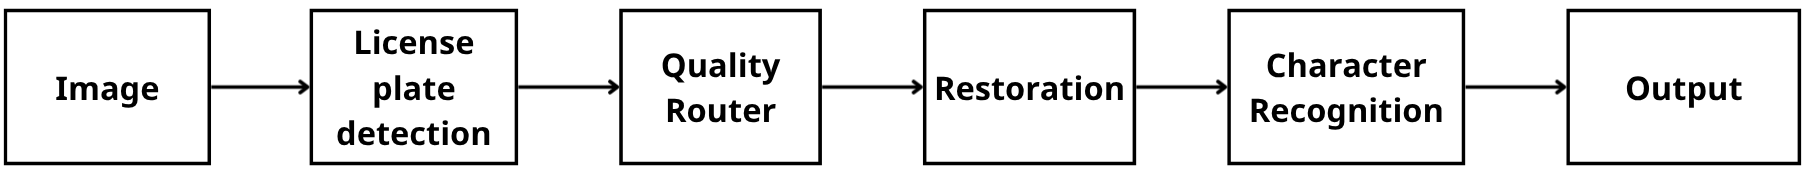
\includegraphics[width=\linewidth, height=3cm]{Images/image_1.png}
		\caption{Block diagram of the proposed adaptive ALPR pipeline. The \textit{QAM} enables conditional routing: clear plates bypass restoration, restorable plates are enhanced via \textit{Swin2SR}, and unrestorable plates are rejected to prevent error propagation.}
		\label{fig:pipeline}
	\end{figure}
	
	\subsection{\textit{Data Preparation}}
	Due to the scarcity of a comprehensive, end-to-end dataset covering all degradation scenarios for Vietnamese license plates, we constructed four specialized datasets corresponding to the specific requirements of each module.
	
	\subsubsection{Dataset-1: Detection (Real-world)}
	We collected and annotated a dataset of \textbf{4,000 images} from Vietnamese traffic surveillance cameras and dashcams. The dataset covers diverse conditions: daytime, nighttime, rainy weather, and varying distances. Annotations were performed using Supervisely with bounding boxes for license plates. The data is split into 70\% training, 20\% validation, and 10\% testing.
	
	\subsubsection{Dataset-2: Quality Classification (Semi-Automated)}
	From Dataset-1, we extracted 1,500 cropped license plate patches. These patches were manually categorized into three classes ("Clear", "Restorable", "Unrestorable") based on human readability and degradation severity, creating a balanced dataset (500 images per class) to train the MobileNetV3 QAM.
	
	\subsubsection{Dataset-3: Restoration (Synthetic Pairs)}
	Since obtaining paired real-world samples (a degraded plate and its perfectly clear counterpart) is infeasible, we employed a \textbf{synthetic degradation pipeline}. We started with high-quality, rectified license plate images and applied random combinations of:
	\begin{itemize}
		\item \textbf{Blur kernels}: Gaussian blur ($\sigma \in [1, 3]$) and Motion blur (kernel size $k \in [3, 9]$, random angle).
		\item \textbf{Noise}: Additive Gaussian noise and Poisson noise.
		\item \textbf{Geometry}: Perspective warping to simulate skew angles up to $45^\circ$.
	\end{itemize}
	This resulted in a curated paired dataset of \textbf{1,318 samples}. Given the specialized nature of the restoration task, we reserved \textbf{1,308 pairs for training} and \textbf{10 representative pairs} for qualitative testing and visual comparison.
	
	\subsubsection{Dataset-4: Recognition (Mixed)}
	To fine-tune the PARSeq model, we combined real-world cropped images from Dataset-1 (transcribed manually) with 970 synthetically generated Vietnamese license plates using the specific fonts and layouts (1-line and 2-line formats) mandated by Vietnamese traffic regulations.
	
	\subsection{\textit{License Plate Detection (Module 1)}}
	
	The primary objective of this module is to accurately localize all license plate instances within a full-frame input image, enabling robust downstream processing under real-world traffic conditions.
	
	\begin{itemize}
		\item \textbf{Model Selection}: We adopt \textit{YOLOv8-nano}~\cite{Yaseen2024WhatIY} as the detection backbone, building upon the foundational real-time object detection paradigm introduced in YOLO~\cite{redmon2016}. This variant is selected for its optimal trade-off between inference speed and accuracy. 
		
		\textbf{Performance Justification:} Empirical validation on our dataset confirms the efficiency of this choice. The model achieves near-perfect detection rates with a \textbf{Recall of 98.3\%} and a \textbf{Mean Average Precision (mAP@50) of 99.4\%} (mAP@50-95: 90.2\%). Crucially for real-time deployment, the total processing latency is minimal, averaging just \textbf{3.6ms} for inference (plus 2.2ms pre-processing and 2.1ms post-processing per image). This ensures the system can handle high-speed traffic flows without bottlenecks.
		
		Fine-tuning on a diverse dataset of annotated Vietnam traffic images further enhances robustness to regional plate variations and imaging distortions~\cite{Nguyen2025AnIO,TranAnh2023LicensePR}.
	\end{itemize}
	
	\begin{figure}[H]
		\centering
		\includegraphics[width=\linewidth]{Images/yolov8_archi.png}
		\caption{The YOLOv8 architecture. Ideally suited for edge deployment, it utilizes a CSPDarknet53 backbone and a path aggregation network (PANet) neck for multi-scale feature fusion \cite{Yaseen2024WhatIY}.}
		\label{fig:yolo_archi}
	\end{figure}
	
	\begin{itemize}
		\item \textbf{Input and Output}: The module accepts a full-resolution input image $I \in \mathbb{R}^{H \times W \times 3}$ and outputs a set of bounding boxes $B = \{(x_{1,i}, y_{1,i}, x_{2,i}, y_{2,i}, c_i)\}_{i=1}^{N}$, where $N$ is the number of detected plates and $c_i$ denotes confidence score. Non-maximum suppression (NMS) with IoU threshold 0.4 eliminates redundant detections.
	\end{itemize}
	
	\begin{figure}[H]
		\centering
		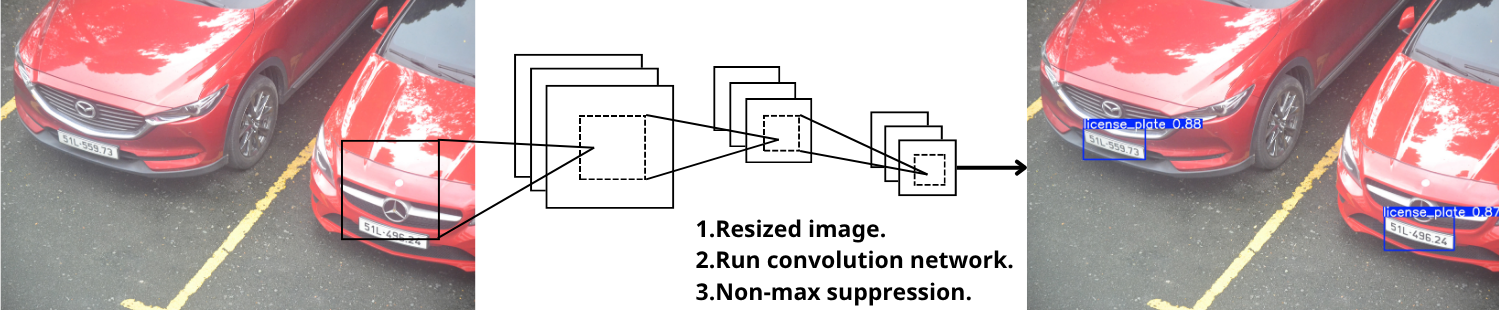
\includegraphics[width=\linewidth]{Images/image_2.png} 
		\caption{The YOLO detection pipeline tailored for Module 1. The process involves resizing, convolutional feature extraction, and bounding box refinement via Non-Maximum Suppression (NMS) \cite{redmon2016}.}
		\label{fig:yolo_pipeline}
	\end{figure}
	
	\begin{itemize}
		\item \textbf{Data Flow}: For each bounding box $B_i$, the corresponding plate region $P_i = \text{crop}(I, B_i)$ is extracted and resized to a fixed dimension ($128 \times 64$) while preserving aspect ratio via padding. These cropped patches serve as direct input to Module 2: Image Quality Assessment and Routing (QAM), enabling adaptive processing based on degradation severity.
	\end{itemize}
	
	\begin{figure}[H]
		\centering
		\includegraphics[width=\linewidth]{Images/yolov8_outputs.jpg}
		\caption{Qualitative results of Module 1. The fine-tuned YOLOv8-nano model successfully localizes license plates with high confidence (e.g., 0.996 precision) under various challenging conditions, including different viewing angles, distances, and vehicle types.}
		\label{fig:yolo_output}
	\end{figure}
	
	\subsection{\textit{Image Quality Assessment and Routing (Module 2)}}
	
	This module represents the core component of the proposed adaptive framework. Instead of processing every detected plate uniformly, this module functions as an intelligent router. Its primary task is to perform Blind Image Quality Assessment (BIQA), a concept explored in various deep learning contexts \cite{simone2017,nima2018}, to determine the optimal subsequent processing path. This adaptive routing is critical for both maximizing accuracy and optimizing computational throughput.
	
	\subsubsection{Model Selection for High-Throughput Routing}
	
	The QAM must be exceptionally fast, as it analyzes every detected plate. A heavy or slow model at this stage would create a significant bottleneck for the entire system. Therefore, a lightweight Convolutional Neural Network (CNN) is required, echoing recent trends in efficient IQA model design \cite{lariqa,javad2025}.
	
	To enable this adaptive processing, we evaluated several candidate backbones: ResNet50, MobileNetV2 \cite{Sandler2018MobileNetV2IR}, EfficientNet-B0 \cite{Tan2019EfficientNetRM}, and MobileNetV3 \cite{Qian2021MobileNetV3FI}. We selected \textbf{MobileNetV3-Small} due to its superior efficiency on edge devices, achieving 3.2$\times$ fewer parameters and 2.8$\times$ lower FLOPs than EfficientNet-B0 while maintaining comparable classification accuracy.
	
	This model is specifically engineered for high performance in resource-constrained environments \cite{Qian2021MobileNetV3FI}. It achieves its efficiency through novel architectural components such as the inverted residual linear bottleneck, a concept introduced in MobileNetV2 \cite{Sandler2018MobileNetV2IR} and refined with h-swish activation functions. This architecture, detailed in Figure~\ref{fig:mobilenet_architec}, provides a superior trade-off between accuracy and latency, making it an ideal choice for our rapid classification task.
	
	\begin{figure}[H]
		\centering
		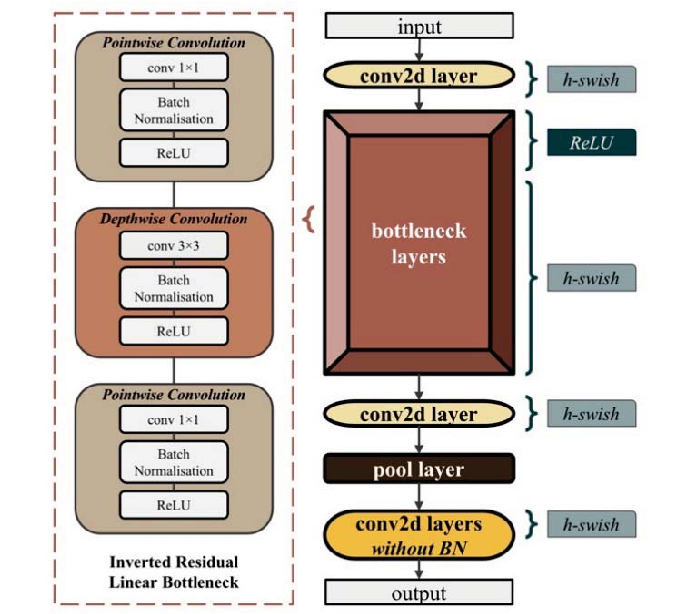
\includegraphics[width=\linewidth, height=4.5cm]{Images/image_4.png}
		\caption{The general architecture of MobileNetV3, illustrating the inverted residual linear bottleneck blocks that enable its computational efficiency \cite{Qian2021MobileNetV3FI}.}
		\label{fig:mobilenet_architec}
	\end{figure}
	
	\subsubsection{Classification Task and Routing Logic}
	
	The QAM is trained as a 3-class classifier. It accepts the cropped license plate image from Module 1 and assigns it to one of three categories:
	\begin{enumerate}
		\item \textbf{"Clear"}: Images with high resolution and sharp focus.
		\item \textbf{"Restorable"}: Images with moderate degradation (blur, glare, skew) recoverable by Module 3.
		\item \textbf{"Unrestorable"}: Severely degraded images (extreme low res, heavy occlusion) to be rejected.
	\end{enumerate}
	
	This classification dictates the system's adaptive data flow, as illustrated in Figure~\ref{fig:module2_pipeline}.
	
	\begin{itemize}
		\item \textbf{Input}: Cropped plate image $P_i \in \mathbb{R}^{128 \times 64 \times 3}$.
		\item \textbf{Output}: Class label $L_i \in \{\text{Clear, Restorable, Unrestorable}\}$.
	\end{itemize}
	
	\begin{figure}[H]
		\centering
		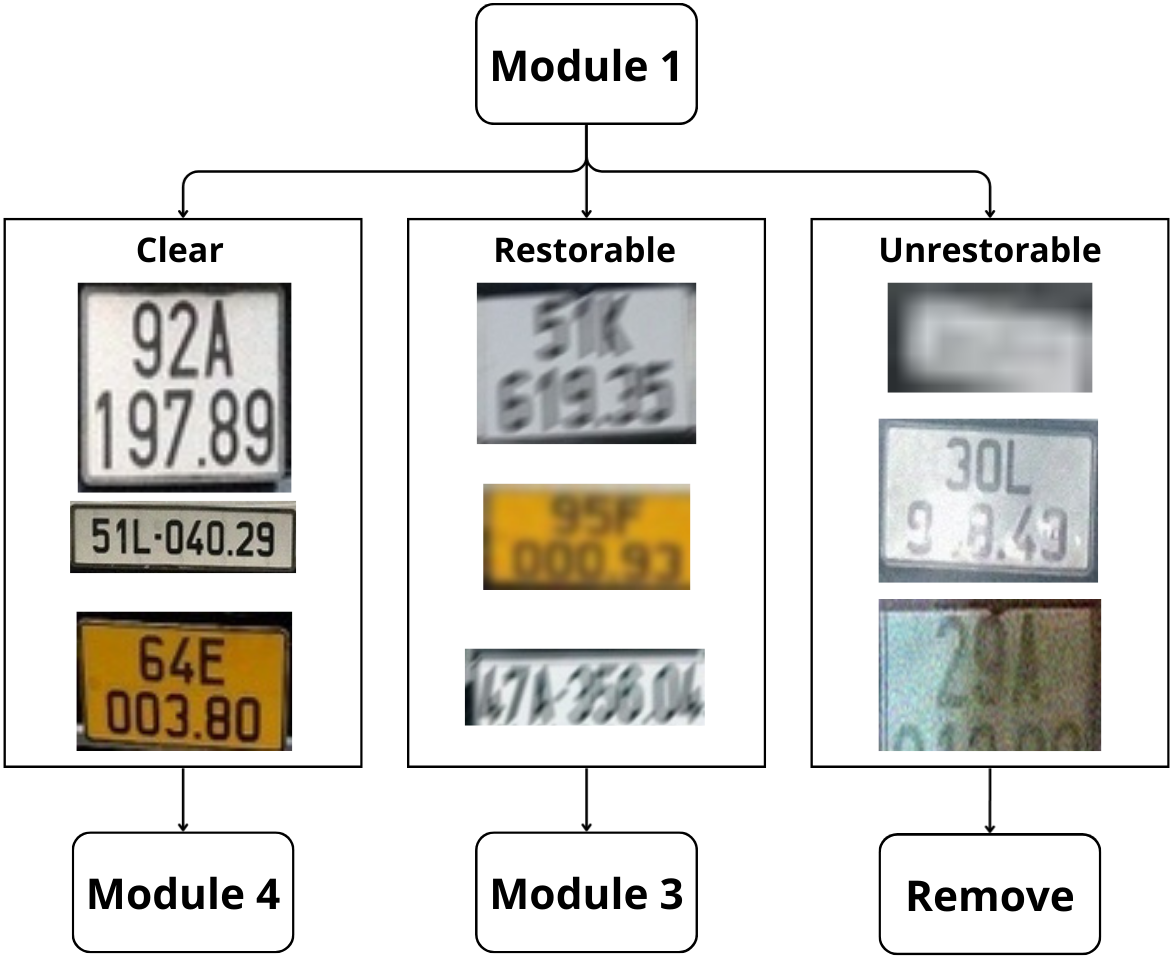
\includegraphics[width=\linewidth]{Images/image_3.png}
		\caption{The 3-branch conditional routing logic of the QAM, illustrated with representative real-world samples. Based on the classification, an image is either sent for recognition, restoration, or removed to optimize system performance.}
		\label{fig:module2_pipeline}
	\end{figure}
	
	\subsubsection{Performance Evaluation}
	
	The Quality Assessment Module was trained using the Cross-Entropy Loss function with an initial learning rate of $0.001$. The model was evaluated on a balanced test set of 150 images (50 images per class).
	
	As shown in the quantitative results, the model achieved an \textbf{Overall Test Accuracy of 88.67\%}. The per-class performance is detailed below:
	
	\begin{itemize}
		\item \textbf{Clear Class}: Achieved a high \textbf{Recall of 98\%} (49/50 correctly identified). This is crucial to ensure that high-quality images are almost never mistakenly sent to the restoration pipeline or rejected.
		\item \textbf{Restorable Class}: Achieved an \textbf{F1-score of 0.92}, indicating a strong ability to correctly identify candidates for restoration.
		\item \textbf{Unrestorable Class}: Precision was \textbf{91\%}, ensuring that the system effectively filters out non-viable inputs without discarding usable data.
	\end{itemize}
	
	The confusion matrix in Figure~\ref{fig:confusion_matrix_m2} further illustrates these results. The minimal off-diagonal elements confirm the robustness of MobileNetV3-Small as an efficient and accurate router for the ALPR pipeline.
	
	\begin{figure}[H]
		\centering
		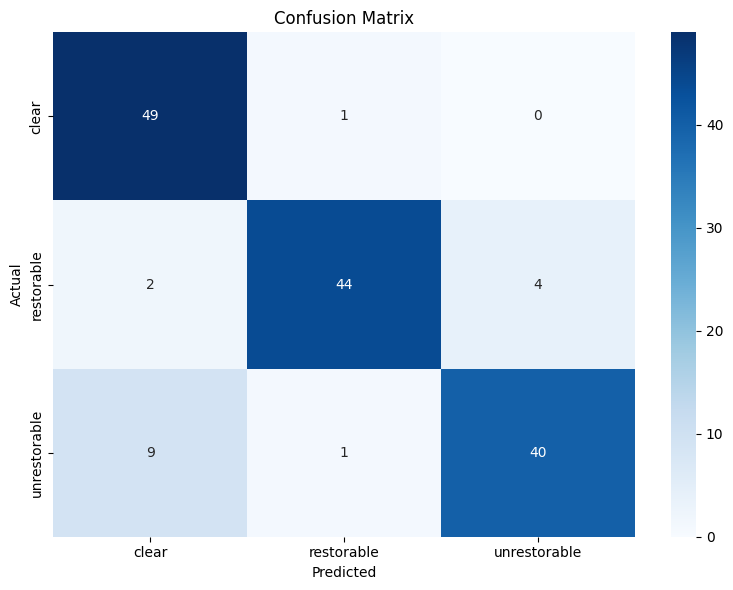
\includegraphics[width=0.8\linewidth]{Images/confusion_matrix_m2.png}
		\caption{Confusion Matrix of the Quality Assessment Module on the test set. The high diagonal values demonstrate the model's effectiveness in distinguishing between clear, restorable, and unrestorable plates.}
		\label{fig:confusion_matrix_m2}
	\end{figure}
	
	\subsection{\textit{Conditional Image Restoration (Module 3)}}
	
	This module serves as the remedial branch of our pipeline, activated exclusively when the QAM (Module 2) classifies an input as "Restorable". The primary objective is to recover textual legibility from degraded patches, ensuring that the structural integrity of characters is preserved for the downstream OCR task.
	
	\subsubsection{Model Selection and Architecture}
	
	As analyzed in Section 2.3 (Related Work), while generative models like GANs offer superior perceptual quality, they pose a significant risk of introducing hallucinated artifacts—fabricating details that do not exist. In the context of license plate recognition, such artifacts are unacceptable as they lead to character misclassification.
	
	Consequently, we prioritize structural fidelity and adopt \textbf{Swin2SR} \cite{conde2022swin2sr} as the restoration backbone. Swin2SR leverages the hierarchical Swin Transformer V2 architecture, incorporating compressed super-resolution layers to process images efficiently. This choice is driven by two key advantages:
	\begin{enumerate}
		\item \textbf{Text Preservation}: The self-attention mechanism in Swin Transformer blocks excels at capturing long-range dependencies, allowing the model to reconstruct high-frequency details (edges of characters) from low-resolution or blurry inputs without distorting the underlying structure.
		\item \textbf{Efficiency}: The compressed architecture is optimized for lower latency compared to standard Vision Transformers, satisfying the throughput requirements of our multi-stage pipeline.
	\end{enumerate}
	
	The detailed architecture of the deployed Swin2SR model is illustrated in Figure~\ref{fig:m3_architec}.
	
	\begin{figure}[H]
		\centering
		\includegraphics[width=\linewidth]{Images/img_m3_architec.png}
		\caption{The architecture of the proposed Swin2SR backbone. It utilizes Swin Transformer blocks for feature extraction and image reconstruction \cite{conde2022swin2sr}.}
		\label{fig:m3_architec}
	\end{figure}
	
	\subsubsection{Technical Implementation}
	
	The restoration module was implemented using the PyTorch framework. The specific configurations and training strategies are detailed below:
	
	\begin{itemize}
		\item \textbf{Input/Output}: The module accepts a degraded image patch $I_{deg} \in \mathbb{R}^{128 \times 64 \times 3}$ and outputs a rectified, clean image $I_{res} \in \mathbb{R}^{128 \times 64 \times 3}$.
		
		\item \textbf{Loss Function}: To maximize character sharpness, we employed the \textbf{L1 Loss} (Mean Absolute Error). Unlike L2 Loss (MSE), which tends to produce overly smooth textures, L1 Loss effectively preserves the high-frequency edge details required for accurate OCR.
		
		\item \textbf{Training Configuration}: The model was trained for \textbf{500 epochs} using the Adam optimizer with an initial learning rate of $2 \times 10^{-4}$. We utilized a cosine annealing learning rate scheduler to stabilize convergence.
		
		\item \textbf{Model Selection}: The training process was monitored using the Peak Signal-to-Noise Ratio (PSNR) metric on a held-out validation set \cite{conde2022swin2sr}. The final model checkpoint was selected based on the best validation performance, achieving a PSNR of \textbf{27.39 dB}, which indicates a significant recovery of image quality sufficient for OCR legibility.
	\end{itemize}
	
	\subsubsection{Experimental Results}
	
	The efficacy of the restoration module was evaluated on a held-out validation set. Quantitatively, the model achieved a Peak Signal-to-Noise Ratio (PSNR) of \textbf{27.39 dB}, indicating significant recovery of image signal.
	
	Qualitatively, as shown in Figure~\ref{fig:m3_results}, the model successfully removes severe motion blur and noise artifacts. Crucially, the restored characters exhibit sharp boundaries and high contrast, significantly improving readability compared to the degraded inputs.
	
	\begin{figure}[H]
		\centering
		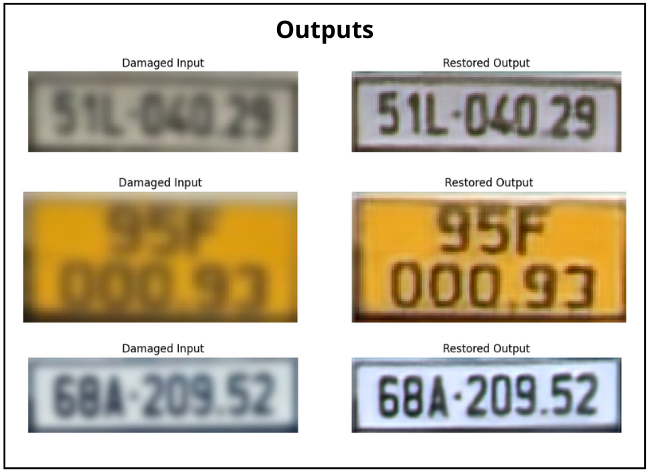
\includegraphics[width=\linewidth]{Images/m3_output_results.png}
		\caption{Qualitative results of the Conditional Restoration Module. The top row displays degraded inputs classified as "Restorable", while the bottom row shows the corresponding outputs restored by Swin2SR, demonstrating enhanced clarity and legibility.}
		\label{fig:m3_results}
	\end{figure}	

	\subsection{\textit{Character Recognition and Retrieval (Module 4)}}
	
	The final module is responsible for transcribing the character string from the processed plate images (either "clear" originals or "restored" outputs from Module 3).
	
	\subsubsection{Model Architecture: ResNet18-PARSeq Hybrid}
	
	As discussed in Section~\ref{related_m4}, to maximize robustness against non-linear distortions, we transition from purely sequential RNN-based models to a Transformer-based approach. Specifically, we construct a hybrid architecture that leverages the strengths of Convolutional Neural Networks (CNNs) for visual feature extraction and Transformers for semantic decoding.
	
	\paragraph{Visual Feature Extraction (ResNet18):}
	Instead of using heavy Vision Transformers (ViT) for the encoder stage, we employ ResNet18 \cite{He2015DeepRL} as the visual backbone. ResNet18 is chosen for its proven efficiency in extracting hierarchical spatial features from images while maintaining a relatively low parameter count compared to deeper variants (e.g., ResNet50 or ViT-Base). The residual skip connections allow the model to preserve signal integrity during the deep feature extraction process, which is critical for distinguishing structurally similar characters (e.g., '8' vs 'B').
	
	\paragraph{Sequence Modeling (PARSeq):}
	The visual features map generated by ResNet18 is then fed into the PARSeq \cite{Bautista2022SceneTR} decoder. Unlike traditional autoregressive models that read strictly left-to-right, PARSeq utilizes Permuted Autoregressive modeling. By leveraging the context-aware nature of Transformer attention mechanisms, it learns an internal language model of license plates, making it inherently robust to partial occlusions and artifacts that typically confuse standard CRNNs.
	
	\subsubsection{Image Processing and Augmentation Strategy}
	
	To further enhance the model's generalization capability on the "wild" Vietnamese dataset, we implemented a rigorous image processing and augmentation pipeline prior to training.
	Based on standard digital image processing principles \cite{Gonzalez2018DigitalIP}, input images are normalized and resized to a fixed height of 32 pixels while maintaining the aspect ratio.
	Furthermore, we employ an aggressive data augmentation strategy \cite{Shorten2019ASO} to simulate real-world degradations. This includes:
	\begin{itemize}
		\item \textbf{Photometric Distortions}: Random brightness, contrast, and saturation adjustments to mimic varied lighting conditions.
		\item \textbf{Geometric Transformations}: Random rotation ($\pm 10^\circ$), shear, and perspective warping to simulate camera misalignments.
		\item \textbf{Noise Injection}: Gaussian blur and iso-noise are added to replicate sensor noise in low-light environments.
	\end{itemize}
	
	\begin{itemize}
		\item \textbf{Input}: A processed license plate image $P_{final} \in \mathbb{R}^{128 \times 32 \times 3}$.
		\item \textbf{Output}: The recognized text string $S$.
		\item \textbf{Data Flow}: The string $S$ serves as the primary key to retrieve vehicle metadata.
	\end{itemize}
	
	\subsubsection{Training Dynamics and Performance}
	
	The model was fine-tuned on the mixed dataset using the optimization strategy described above. As illustrated in Figure~\ref{fig:m4_training}, the training loss decreases consistently while accuracy metrics improve, validating the stability of the ResNet-PARSeq hybrid.
	
	We evaluate the model using two primary metrics:
	\begin{enumerate}
		\item \textbf{Character Accuracy (Char Acc)}: The percentage of individual characters correctly predicted.
		\item \textbf{Sequence Accuracy (Seq Acc)}: The percentage of plates where the \textit{entire} string is predicted correctly.
	\end{enumerate}
	
	At the best checkpoint (Epoch 70), the model achieved a Character Accuracy of 96.07\% and a Sequence Accuracy of 89.69\%. This high sequence accuracy demonstrates the model's ability to capture the global context of Vietnamese license plates effectively.
	
	\begin{figure}[H]
		\centering
		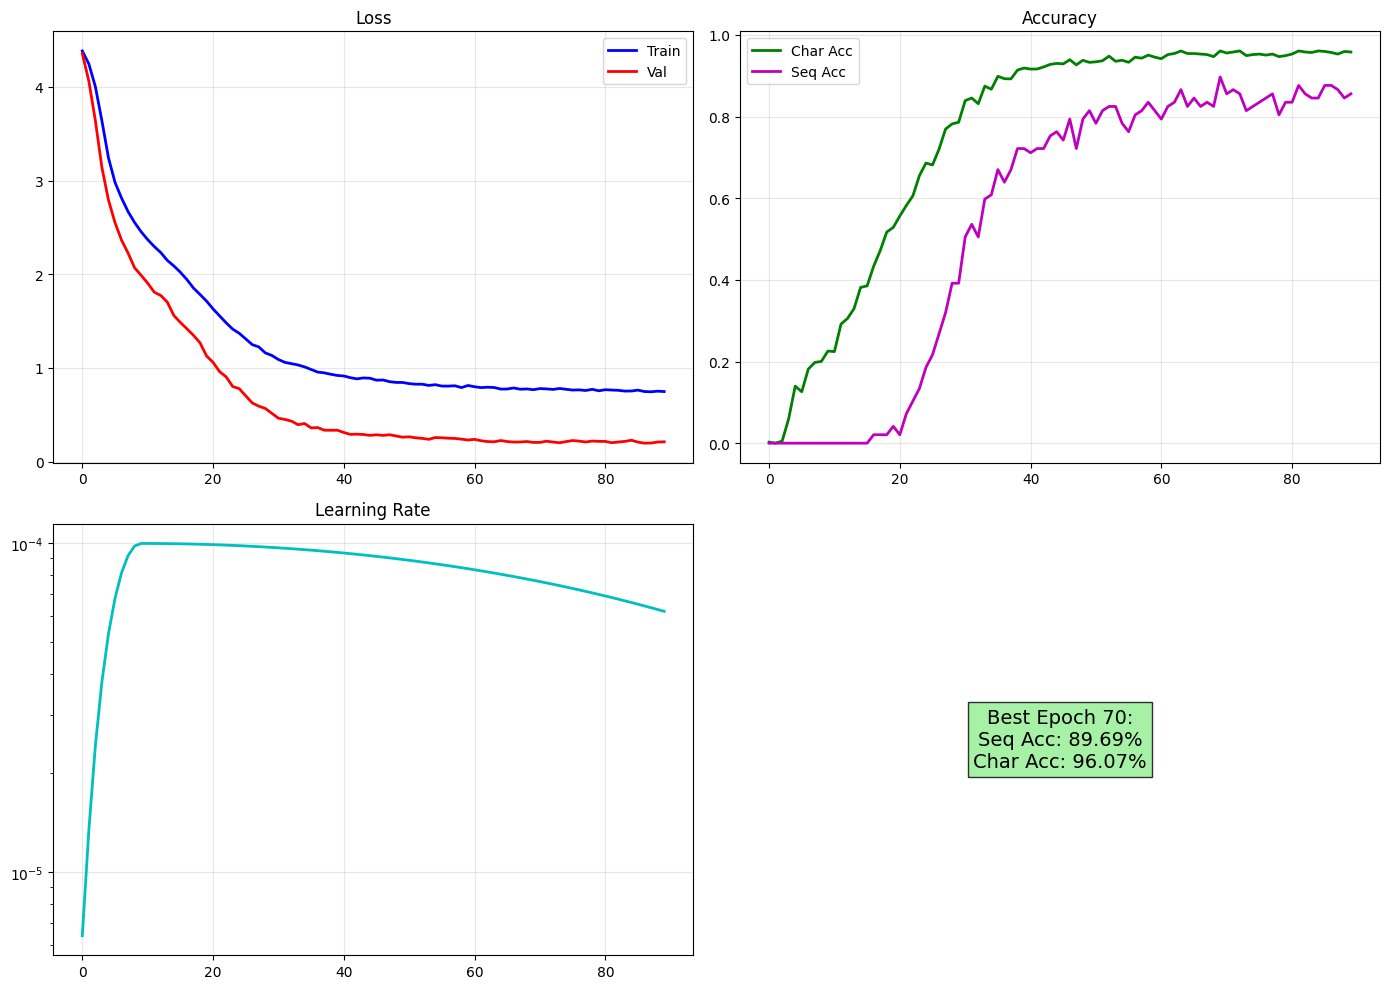
\includegraphics[width=\linewidth]{Images/training_info_m4.png}
		\caption{Training dynamics of Module 4. The graphs show the loss convergence, the improvement in Character and Sequence accuracy over epochs, and the learning rate schedule.}
		\label{fig:m4_training}
	\end{figure}
	
	Qualitative results are presented in Figure~\ref{fig:m4_pred}. The model demonstrates high robustness, correctly recognizing plates even with complex backgrounds or slight skew.
	
	\begin{figure}[H]
		\centering
		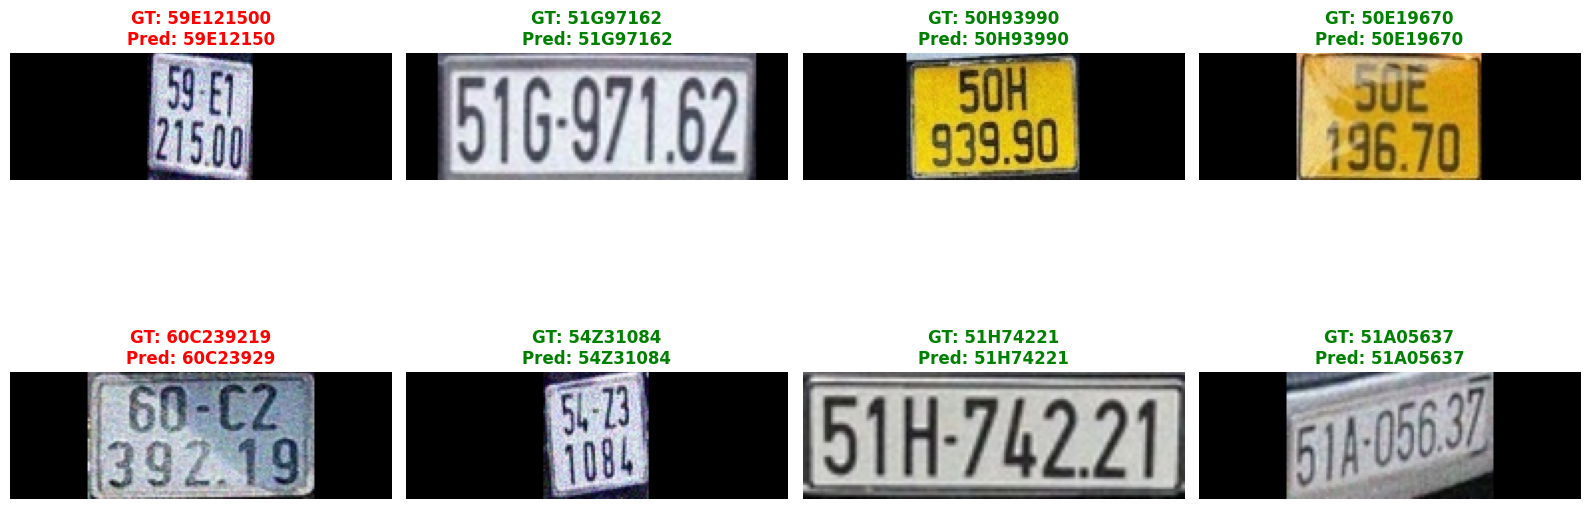
\includegraphics[width=\linewidth]{Images/pred_with_gt_m4.png}
		\caption{Qualitative evaluation of the PARSeq model (ResNet18 Backbone). Green text indicates correct predictions; red text indicates errors compared to Ground Truth (GT).}
		\label{fig:m4_pred}
	\end{figure}
	
	\begin{figure}[H]
		\centering
		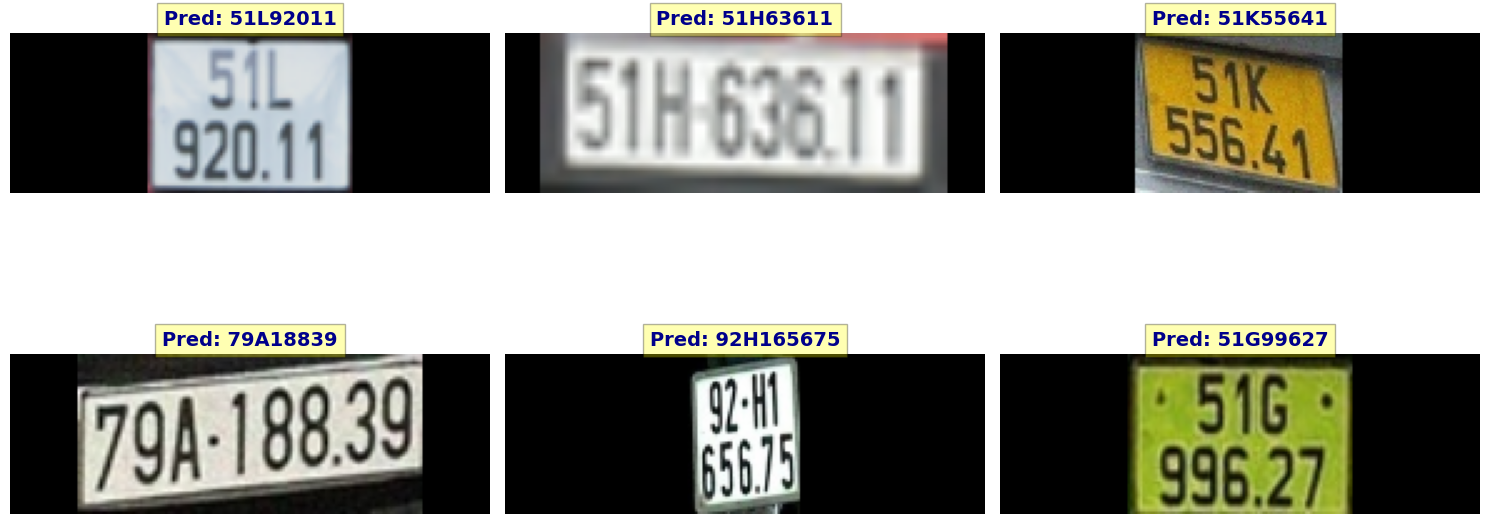
\includegraphics[width=\linewidth]{Images/pred_no_gt_m4.png}
		\caption{Inference results without Ground Truth.}
		\label{fig:m4_inference}
	\end{figure}
	
	
	\section{CONCLUSION AND FUTURE WORK}
	
	\subsection{Conclusion}
	This research presented a novel, adaptive deep learning framework for Automatic License Plate Recognition (ALPR), specifically tailored to the diverse and challenging context of Vietnamese traffic environments. Unlike traditional monolithic pipelines, our proposed system introduces a lightweight \textbf{MobileNetV3-based} Quality Assessment Module (QAM) that functions as an intelligent router. By dynamically classifying inputs as "clear," "restorable," or "unrestorable," the system optimizes computational resources—selectively applying the computationally intensive Swin2SR restoration only when necessary.
	
	Experimental results demonstrate that this multi-task approach significantly improves OCR accuracy on degraded inputs (blurred, glared, or skewed plates) compared to baseline methods, while maintaining high throughput for clean data. The integration of the \textbf{ResNet-PARSeq hybrid model} further enhances robustness against character-level distortions and occlusions, validating the effectiveness of the proposed end-to-end adaptive pipeline.
	
	\subsection{Limitations}
	Despite the promising results, the current framework has certain limitations. First, the Conditional Restoration Module (Module 3) relies heavily on synthetic data for training due to the scarcity of paired real-world degraded/clean license plate datasets. While effective, synthetic degradations may not perfectly model complex real-world artifacts such as heterogeneous weather conditions (e.g., heavy rain streaks or fog). Second, although the routing mechanism saves resources, the restoration backbone itself (Swin2SR) remains relatively computationally demanding compared to simple interpolation methods, which may pose latency challenges on extremely low-power edge devices (e.g., Raspberry Pi 3 or legacy embedded systems).
	
	\subsection{Future Work}
	Future work will focus on bridging the domain gap between synthetic and real-world data by collecting a larger-scale dataset of real-world degraded plates. Additionally, we aim to optimize the inference efficiency of the restoration module using model quantization and pruning techniques (e.g., \textbf{TensorRT or ONNX Runtime optimization}) to facilitate deployment on constrained edge computing platforms. Finally, extending the framework to incorporate temporal information from video streams could further improve detection and recognition stability in dynamic traffic flow scenarios.
	
	\section{REFERENCES}	
	\begingroup
	\renewcommand{\section}[2]{}  
	\bibliographystyle{ieeetr}
	\bibliography{references}
	\endgroup
\end{document}